\section{Mô phỏng hệ thống mạng}
Mô hình mô phỏng được xây dựng hoàn chỉnh trên phần mềm Cisco Packet Tracer dựa trên kiến trúc thiết kế ở các phần trước. Để đảm bảo sơ đồ trực quan và tránh trùng lặp cấu hình, mỗi phân khu được triển khai với các tầng, khoa và máy trạm đại diện cho các phân mạng (VLAN) chính.

\subsection{Cấu trúc triển khai trên Cisco Packet Tracer}
\begin{itemize}
    \item \textbf{Trụ sở chính:} Triển khai mô hình ba lớp gồm cặp Edge Router (\texttt{ER1}, \texttt{ER2}), cặp thiết bị lọc lưu lượng biên (\texttt{FW1}, \texttt{FW2}), cặp Core Switch (\texttt{CORE1}, \texttt{CORE2}) cấu hình dự phòng Gateway HSRP, khu Server Farm (\texttt{APP\_1}, \texttt{APP\_2}, \texttt{DB\_1}, \texttt{DB\_2}, \texttt{SRV\_STG}, \texttt{INFRA\_1}, \texttt{INFRA\_2}) và vùng DMZ (\texttt{DMZ\_WEB}, \texttt{DMZ\_MAIL}, \texttt{DMZ\_DNS}).
    \item \textbf{Tòa A và Tòa B:} Tòa A sử dụng Distribution Switch \texttt{DS-A} kết nối xuống các Access Switch đại diện (\texttt{AS-A1}, \texttt{AS-A2}) cùng hệ thống Wi-Fi cục bộ. Riêng Tòa B bố trí cặp Distribution Switch dự phòng song song (\texttt{DS-B1}, \texttt{DS-B2}) cho Khoa Cấp cứu (\texttt{PC-CAPCUU}) và Hồi sức tích cực (\texttt{PC-ICU}), đồng thời tách riêng nhánh thiết bị y tế IoT (\texttt{PC-IOT-BED}) và camera giám sát (\texttt{CAM-B1}).
    \item \textbf{Hai cơ sở phụ (ĐBP và BHTQ):} Mỗi cơ sở áp dụng mô hình lõi thu gọn với Router biên (\texttt{R-DBP}, \texttt{R-BHTQ}) nối về cặp thiết bị biên tại Trụ sở chính, Switch truy cập, máy trạm đại diện, các máy chủ chuyên biệt (\texttt{SRV-PIS}, \texttt{SRV-CRM}, \texttt{SRV-FIS}, \texttt{SRV-DR}) và điểm phát Wi-Fi riêng (\texttt{WIFI-DBP}, \texttt{WIFI-BHTQ}).
    \item \textbf{Định tuyến và bảo mật:} Cấu hình chia VLAN, đường Trunk 802.1Q giữa các tầng chuyển mạch, định tuyến động OSPF liên cơ sở và áp dụng Extended ACL nhằm cô lập thiết bị IoT khỏi vùng hạ tầng quản trị.
\end{itemize}

\begin{figure}[H]
    \centering
    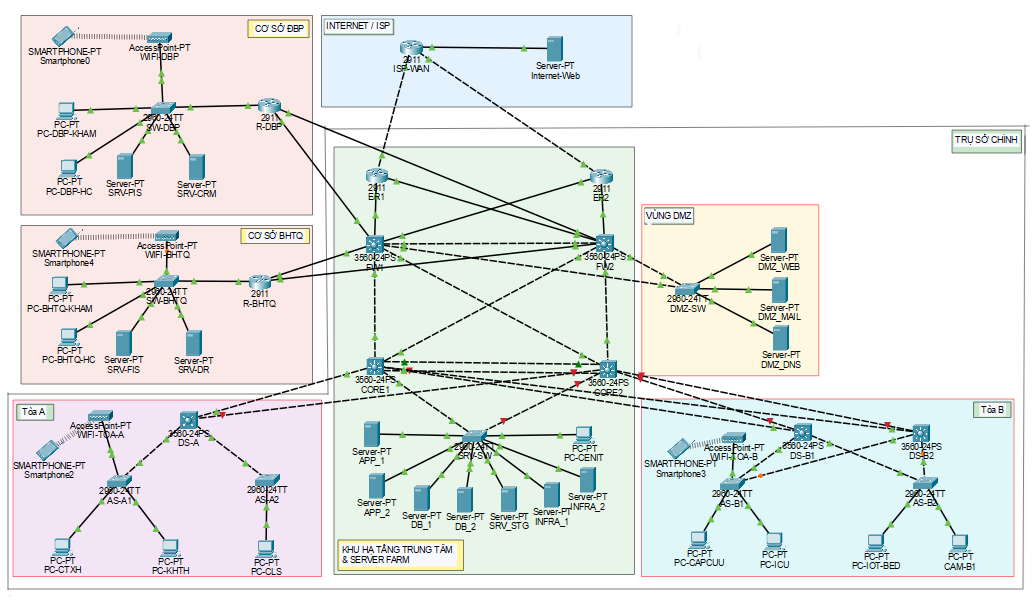
\includegraphics[width=\textwidth]{Assets/tong_quan2.png}
    \caption{Sơ đồ mô phỏng tổng quan kiến trúc mạng bệnh viện trên Cisco Packet Tracer}
    \label{fig:topo_overview}
\end{figure}